\documentclass[12pt, twoside]{article}
\usepackage{jmlda}
\usepackage{amsfonts}
%\usepackage{algorithm}
%\usepackage{algcompatible}
\usepackage{algorithmic}
\usepackage{booktabs,siunitx}
\usepackage{bm}
\usepackage[outline]{contour}
\graphicspath{{../figures/}}

\raggedbottom

\usepackage{float}


\usepackage{algorithm}
\usepackage{lipsum}

\makeatletter
\newenvironment{breakablealgorithm}
  {
   \begin{center}
     \refstepcounter{algorithm}% New algorithm
     \hrule height.8pt depth0pt \kern2pt% \@fs@pre for \@fs@ruled
     \renewcommand{\caption}[2][\relax]{% Make a new \caption
       {\raggedright\textbf{\fname@algorithm~\thealgorithm} ##2\par}%
       \ifx\relax##1\relax % #1 is \relax
         \addcontentsline{loa}{algorithm}{\protect\numberline{\thealgorithm}##2}%
       \else % #1 is not \relax
         \addcontentsline{loa}{algorithm}{\protect\numberline{\thealgorithm}##1}%
       \fi
       \kern2pt\hrule\kern2pt
     }
  }{% \end{breakablealgorithm}
     \kern2pt\hrule\relax% \@fs@post for \@fs@ruled
   \end{center}
  }
\makeatother

%\usepackage{algpseudocode}
%\usepackage{array,calc}
%\usepackage{longtable,tabu}
%\usepackage{tabularray}
%\usepackage{caption}
%\usepackage{diagbox}
%\usepackage{multirow}
%\newlength{\dig}
%\settowidth{\dig}{6}


\renewcommand{\thealgorithm}{}

\newcommand{\hdir}{.}



\begin{document}

\English

\title
    [] % short title for page headings, not necessary if a full title fits the headings
    {Influence of hyperparameters on online aggregation with countable experts} % full title
\author
    [S.\,M.~Kunin-Bogoiavlenskii] % short list of the authors (<= 3) for page headings, is necessary only if the full list does not fit the headings
%S.M. Kunin-Bogoiavlenskii, A.V. Zukhba, and R.D. Zukhba
    {S.\,M.~Kunin-Bogoiavlenskii, A.\,V.~Zukhba, R.\,D.~Zukhba, and V.\,V.~V’yugin} % full list of the authors, presented in the table of contetns of the issue
    [S.\,M.~Kunin-Bogoiavlenskii, A.\,V.~Zukhba] % list of the authors presented in the title page of the article, is necessary only if it differs from the full list of the authors in braces, i.e. '{' and '}'
\email
    {kunin-bogoiavlenskii.sm@phystech.edu; a\_\_l@mail.ru}
%\thanks
%    {The research was
%     %partially
%     supported by the Russian Foundation for Basic Research (grants 00-00-0000 and 00-00-00001).}
\organization
    {Moscow Insitute of Physics and Technology}
\abstract
    {

    Aggregating forecasts from multiple experts is a valuable method to improve prediction accuracy.
    This paper examines the influence of hyperparameters on the accuracy of the aggregation algorithm for a countable number of experts.
    We implement a time series generator with specified properties and an aggregating forecasting model. 
    We conduct a series of experiments with various hyperparameters of the algorithm (including initialization weights, mixing scheme, train window). 
    The experiments confirm that these hyperparameters have a significant influence on the algorithm's performance.           
        
%   \noindent
%   \textbf{Background}:    One paragraph about the problem, existent approaches and its limitations.
%   
%   \noindent
%   \textbf{Methods}: One paragraph about proposed method and its novelty.
%   
%   \noindent
%   \textbf{Results}: One paragraph about major properties of the proposed method and experiment results if applicable.
%   
%   \noindent
%   \textbf{Concluding Remarks}: One paragraph about the place of the proposed method among existent approaches.
%               
    \noindent
        \textbf{Keywords}: \emph{online learning; aggregating algorithm; prediction with experts’ advice; Fixed Share, Mixing Past Posteriors (MPP)}}

%these fields are filled in by the journal editors
%\doi{10.21469/22233792}
%\receivedRus{01.01.2017}
\receivedEng{January 01, 2017}

\maketitle
%\linenumbers

\section{Introduction}
%\noindent %this command is placed at the beginning of the first sentence of each paragraph/section only.
This work is inspired by the algorithm, developed in the article \cite{article}, considering online game of prediction with experts' advice. The data is presented as a time series, consisting of outcome pairs --- <<signal>> and <<response>>. 
In contrast to the classical statistical theory of sequential prediction, we make no assumptions about the nature of the data (which could be deterministic, stochastic, etc.). 
We use machine learning methods to build forecasters within a game-theoretic approach.
The online learning master model considers a series of reference forecasters, referred to as experts, to build its opinion by combining their predictions.


%\noindent
The general prediction algorithm with expert advice follows this structure:
Learning progresses in trials at discrete points in time. 
During each step , expert models, based on past observational data subsamples, provide their predictions. 
The master model then makes a decision using the chosen aggregating algorithm. 
At the end of the trial, the generator presents the true outcome, and both the master and expert models are scored using a loss function. 
The difference between the master's cumulative losses and the expert's cumulative losses is defined as regret.
The traditional goal of the aggregating algorithm is to keep it as small as possible.

%\noindent
We use special assumptions about the data generation structure when building forecasting strategies. 
It is assumed that there are multiple generators, whose structure is unknown to the predictors. 
The time series is obtained by merging segments, each produced by one of the generators. 
These segments are called areas of stationarity, and can be studied using machine learning methods.
%These generators switch, producing a time series that is subdivided into a sequence of segments --- areas of stationarity, which can be studied using machine learning methods. 
Each corresponding local predictive model will be constructed based on data from the area of stationarity and can be then successfully applied in other areas of stationarity generated by the same generator.

%\noindent
In this formulation of the forecasting problem, the series of prediction steps is divided into segments that frame arbitrary sequences of expert strategies. 
The sequence of segments and its associated sequence of experts is called a partition. 
The modified goal of the aggregating algorithm is to perform well relative to the best partition. 
Accordingly, the new concept of algorithm regret is the difference between the algorithm's losses and the cumulative losses of the sequence of experts. 
This change allows for a more accurate modeling of real-life conditions, where the nature of responses may change over time and different experts may predict with varying degrees of success depending on the current trend. 

%\noindent
The corresponding algorithm is called Fixed Share \cite{article98}. 
A further proposed generalization of it is the Mixing Past Posteriors (MPP) method \cite{article02}. 
The cumulative losses of the aggregating algorithm are related to convex combinations of expert losses. 
The concept of regret also changes. 
Now the algorithm's cumulative losses are compared to the cumulative losses of convex combinations of expert strategies.

A characteristic feature of the problem considered in \cite{article} is the absence of a predefined set of competing expert strategies, as was the case in the works cited above.
Instead, new expert strategies are constructed at each step of the online learning process.
The master must aggregate the forecasts of all expert strategies constructed up to that time in real-time at each step. 
Algorithm GMPP, proposed in \cite{article}, is the foundation of our experiments. 

\section{Problem statement}
%\paragraph{Definitions}
Let $x_1, x_2, \dots$ be the sequence of signals belonging to the sample space  $\mathcal{X}$. 
The masters goal is to predict the sequence of the corresponding responces $y_1, y_2, \dots$ belonging to the outcome space $\mathcal{Y}$. 
We assume that the master knows $a, b \in \RR$ --- the bounds of the responces sequence, s.t. $\forall i\quad a \leq y_i \leq b$.

We assume that there is an countable number of experts $i \in \mathcal{N}$, where $\mathcal{N}$ is the natural numbers set. 
The predictions of the master and experts belong to the decision space $\mathcal{D}$. 
Let $ \lambda: \mathcal{D} \times \mathcal{Y} \rightarrow \RR_+$ be the nonnegative loss function. 

At each step $t$ every expert $i \in \mathcal{N}$ provides his prediction $f_t^i = f_t^i(x_t)  \in \mathcal{D}$. 
After obtaining them the master gives his prediction $p_t = p_t(x_t) \in \mathcal{D}$. 
Next, the generator reveals the true outcome $y_t$, and the losses are computed.
Let $h_t = \lambda(p_t, y_t)$ be the master's loss , and $l_t^i = \lambda(f_t^i, y_t)$ be the loss of expert $i \le t$. For $i > t$ (i.e. expert $i$ is not yet initialized), $l_t^i = h_t$.

With designations $L_T^i = \sum_{t = 1}^T l_t^i$, representing the cumulative loss of expert $i$ during the first T steps, and $H_T = \sum_{t = 1}^T h_t$, 
representing the master's cumulative loss during the first T steps, we can define the master's regret relative to the expert $i$ as $R^i_T = H_T - L^i_T$. 

The best partition is formed based on a hindsight analysis of the experiment results, assuming we know the segment boundaries. For each segment, the best partition predictions are set equal to the predictions of the best local expert (the one that has the lowest cumulative sum on that segment). Master's regret relative to the best partition is defined as $R_T= H_T - L_T$, where $L_T$ is the cumulative loss of the best partition. We use this $R_T$ as a metric in our experiments.

 
%\paragraph{Aggregating algorithm}
\vspace{5mm}

\begin{breakablealgorithm}
\caption{GMPP}
\begin{algorithmic}
%\STATE Parameters:
%\STATE \textbullet~ Initialization weights $w^i_1$, s.t. $\sum\limits_{i \in \mathcal{N}}w^i_1 = 1$
%\STATE \textbullet~ Alpha parameter series $\{\alpha_t\}$
%\STATE \textbullet~ Train window size 

\STATE Initialize the weights $w^i_1$ so that $\sum\limits_{i \in \mathcal{N}}w^i_1 = 1$
\FOR{$t = 1, 2, \dots$}

  
\STATE\textbf{\textperiodcentered}~ Expert $f^t$ initialization
\STATE\textbf{\textperiodcentered}~ Signal $x_t$ is received 
\STATE\textbf{\textperiodcentered}~ Experts' predictions $f_t^i = f_t^i(x_t), 1 \le i \le t$ 
\STATE\textbf{\textperiodcentered}~ Computation of normalized weights of experts  $1 \le i \le t$: $\widehat{w}^i_t = \dfrac{w^i_t}{\sum_{j=1}^t w_t^j}$
\STATE\textbf{\textperiodcentered}~ Master's prediction evaluation $\gamma_t = \textit{Subst}(\mathbf{f_t}, \mathbf{\widehat{w}_t}) = \dfrac{a+b}{2} + \dfrac{1}{2\eta(b-a)}\cdot \ln \dfrac{\sum\limits_{i \in \mathcal{N}} \hat w_t^i e^{-\eta(b - f_i)^2}}{\sum\limits_{i \in \mathcal{N}}  \hat w_t^i e^{-\eta(a - f_i)^2}}$, \\ where $\mathbf{\widehat{w}_t} = (\widehat{w}_t^1, \widehat{w}_t^2, \dots \widehat{w}_t^t),\ \mathbf{f_t} = (f_t^1, f_t^2, \dots f_t^t)$
\STATE\textbf{\textperiodcentered}~ True outcome $y_t$ is revealed
\STATE\textbf{\textperiodcentered}~ Computation of master's loss $h_t = \lambda(p_t, y_t) $ and experts' losses: $l_t^i =
\begin{cases}
        \lambda(f_t^i, y_t), & \text{if $i \le t$} \\
        h_t, & \text{if $i > t$}
\end{cases}$
\STATE\textbf{\textperiodcentered}~ \textbf{Loss Update} weights modification
\[  \widetilde{w}_t^i = \dfrac{w_t^i e^{\eta l_t^i}}{\sum\limits_{j = 1}^t w_t^j e^{-\eta l_t^i} + e^{-\eta h_t} (1 - \sum\limits_{j = 1}^t w_t^j) } \]
\STATE\textbf{\textperiodcentered}~ \textbf{Mixing Update} weights modification
\[  \widetilde{w}_{t+1}^i = \alpha_t\widetilde{w}_1^i + (1 - \alpha_t)\widetilde{w}_t^i\] 

\ENDFOR


\end{algorithmic}
\end{breakablealgorithm} 

\section{Experiment}
We implement the synthetic time series generator and the GMPP algorithm itself. 
We then conduct experiments to analyze the effects of varying hyperparameters.
\subsection{Data generation}

We define generators $G_1, G_2, \dots, G_k$ by their weight vectors $\vec w_1, \vec w_2, \dots, \vec w_k \in \RR^d$. 
Here, $d$ represents the dimensionality of the signals.

We generate signals as a series of vectors $\vec x_1, \vec x_2, \dots, \vec x_T \sim \mathcal{N}(0, I_d)$, indicating they are drawn from a zero-mean Gaussian distribution with an identity covariance matrix .

This series of vectors is then randomly divided into a sequence of segments. 
We denote these segments as $S_1, S_2, \dots, S_m$. 
Each segment $S_i$ is a sequence of vectors itself, containing elements from $\vec x_{s_{i-1}+1}$ to $\vec x_{s_i}$ (where $s_i$ is the index of the last element in segment $i$, $s_0 = 0$). 
Importantly, each segment $S_i$ is assigned to a specific generator $G_{g(i)}$ according to a random function $g$. 
This function determines which generator is responsible for creating responses for that segment.

Ultimately, we obtain the series of responses $y_1, y_2, \dots, y_T$ by taking the dot product of each signal vector with the weight vector of the corresponding  generator and adding the noise: $y_i = \langle \vec w_{g(i)}, \vec x_i \rangle + \varepsilon_i,$ where $\varepsilon_i \sim \mathcal{N}(0, \sigma^2)$ 

\vspace{2mm}

In our experiment, we fix the following data characteristics:
\begin{itemize}
\item Time series length $T = 2000$
\item For adequate algorithm behaviour in the beggining of the algorithm, 
we add few segments (one from each generator) in front of the main time series. This part is not taken into account in regret calculation
\item Signals dimention $d=10$
\item Generator weight vectors are drawn from a uniform distribution $U_{[-10, 10]^d}$
\item Responses bounds $(a, b) = (-40, 40)$
\item Segments sizes are drawn from a uniform distribution $U_{[50, 300]}$
\item Number of generators $k = 5$
\item Function g randomly alternates generators for adjacent segments
\item White noise variance $\sigma^2= 1$
\end{itemize}

Also, to ensure robust performance from the outset, we insert a short priming sequence at the beginning of the time series. This sequence includes one segment from each generator. Importantly, the data from this priming sequence is excluded from the regret calculation.
\subsection{Experts}

Each expert $f_t$ is initialized as a linear regression model. 
This model is trained on a fixed window of $l$ past observations. 
The training process yields a weight vector, which is calculated as  
$\theta_t = (\vec X^T\vec X)^{-1}\vec X^T\vec y$,\ where $\vec X^T = (\vec x_{t-1}, \vec x_{t-2}, \dots \vec x_{t-l}),\ \vec y = (y_{t-1}, y_{t-2}, \dots y_{t-l})$. 

Given a new signal vector  $\vec x$, the expert's prediction is obtained by calculating the dot product between the weight vector and the signal vector: $f_t(\vec x) = \langle \vec \theta_t, \vec x \rangle$ 


%\newpage


\subsection{Hyperparameters}

We investigate the impact of various hyperparameters on the GMPP algorithm's performance, focusing on initialization weights, mixing scheme, mixing update coefficients, and expert window size. 
\begin{enumerate}
\item Initialization Weights ($w_1^t$):
\begin{itemize}
\item Default: $w_1^t = \frac{1}{(t+1)\ln^2(t+1)}$
\item Experimental: 
\begin{itemize}
\item $w_1^t = \frac{1}{e^t}$, exploring exponential decay as a common alternative.
\item $w_1^t = \frac{1}{(t+4)\ln(t+4)\ln^2\ln(t+4)}$, representing a slower decaying function.
\item $w_1^t = \frac{1}{t^\alpha}$, with $\alpha \in (1, 2]$, to analyze the impact of faster decay rates.
\item $w_1^t = \frac{1}{t^\alpha}$, with $\alpha \in (0, 1]$, to analyze the behavior with diverging weights.


\end{itemize}
\end{itemize}


%\contourlength{0.1pt}
%\item \contour{black}{Mixing Update Scheme:}

\item Mixing Update Coefficients ($\alpha_t$):
\begin{itemize}
\item Default: $\alpha_t = \frac{1}{t+1}$
\item Experimental: 
\begin{itemize}
\item $\alpha_t = \frac{1}{(t+1)^\beta}$, with $\beta \in (0, 2]$, to analyze different decay speeds.
\item $\alpha_t = \frac{1}{t+c}$, with varying $c$, to analyze the influence of a constant shift.
\item $\alpha_t = \frac{1}{c}$, with $100 \le c \le10000$
\item $\alpha_t = \frac{1}{e^{t/3}}$, exponential decay, rapidly reducing the influence of initial weights.         

\end{itemize}


\end{itemize}

\item Mixing Update Scheme:

While GMPP in \cite{vvbook} utilizes a specific scheme, we explore various Mixing Fixed-Share Update schemes as presented in \cite{article02}:

\[ \widetilde{w}_{t+1}^i = \sum_{q=1}^t\beta_t(q)\widetilde{w}_q^i  \]

\begin{itemize}
\item Start Vector Share (default in GMPP) --- emphasizes the initial weight vector and the most recent update:
    \[\beta_t(q) =
    \begin{cases}
    \alpha_t, & q = 1 \\
    0, & 1 < q < t \\
    1 - \alpha_t, & q = t 
    \end{cases}\]
    
        \item Uniform Past Share ---  assigns equal weight to all past updates : 
            \[\beta_t(q) =
            \begin{cases}
            \alpha_t\frac{1}{t}, & 1 \le q < t \\
            1 - \alpha_t, & q = t 
            \end{cases}\]
            
        \item Decaying Past Share ---  assigns decreasing weights to past updates:
            \[\beta_t(q) =
            \begin{cases}
            \alpha_t\frac{1}{(t-q)^\gamma}\frac{1}{Z_t}, & 1 \le q < t \\
            1 - \alpha_t, & q = t
            \end{cases}\]
            \hfill ,with $Z_t = \sum_{q=0}^{t-1} \frac{1}{(t-q)^\gamma}, \gamma > 0$. 
        
\end{itemize}



\item Window Size ($l$): We vary train window size $l \in \{5, 10, 20, 50, 100\}$ to check algorithm performance in situations when experts lack information or when they often train on pieces made by different generators.

\end{enumerate}

As a metric of quality we use $R_T$ --- master's regret relative to the best partition.
We run experiments 4 times for each configuration of hyperparameters, and take the mean of the earned regrets.

\subsection{Results}
%\section{Results}


\begin{table}[h]
\centering

\begin{tabular}{ccr}

\toprule
Weight function & Regret \\
\midrule
$1 / ((t+1)\ln^2(t+1))$   & 136360.61 \\
$1 / t^{1.01}$  &\ 94758.81 \\
 $1 / t^{1.1}$&\ 98359.26 \\
$1 / t^{2}$ & 113298.39 \\
%$1/ e^{x/4}$ & 425358.37 \\
$1 / ((x + 4) * \ln(x + 4) * \ln^2\ln(x + 4)) $  & 127634.11 \\
\bottomrule
\end{tabular}
\caption{Regret value for different weight functions} \hspace{16cm}
\end{table}


\begin{table}[h]
\centering
\begin{tabular}{r|ccc}
 &
\multicolumn{2}{c}{Weight function} \\
\toprule {Window size}  &

\centering $\dfrac{1}{(t+1)\ln^2(t+1)}$ &
\centering $\dfrac1{t^{1.01}}$  & \tabularnewline

\midrule
5 &  188586.09 & 141788.84 \\ %& 113612.93 \\
10 &  136360.61 &\ 94758.81 \\ %&\ 83776.19 \\
20 &  129543.68 &\ 93456.18 \\ %& 114114.46 \\
50 &  143610.19 &\ 97600.05 \\ %& 123485.38 \\
100 & 151434.18 & 101551.31 \\ %& 126436.54 \\
200 & 164746.91 & 113835.86 \\ %& 137111.18 \\
\bottomrule
\end{tabular}
\caption{Dinamics of regret value over different sizes of train window} \hspace{16cm}

\end{table}


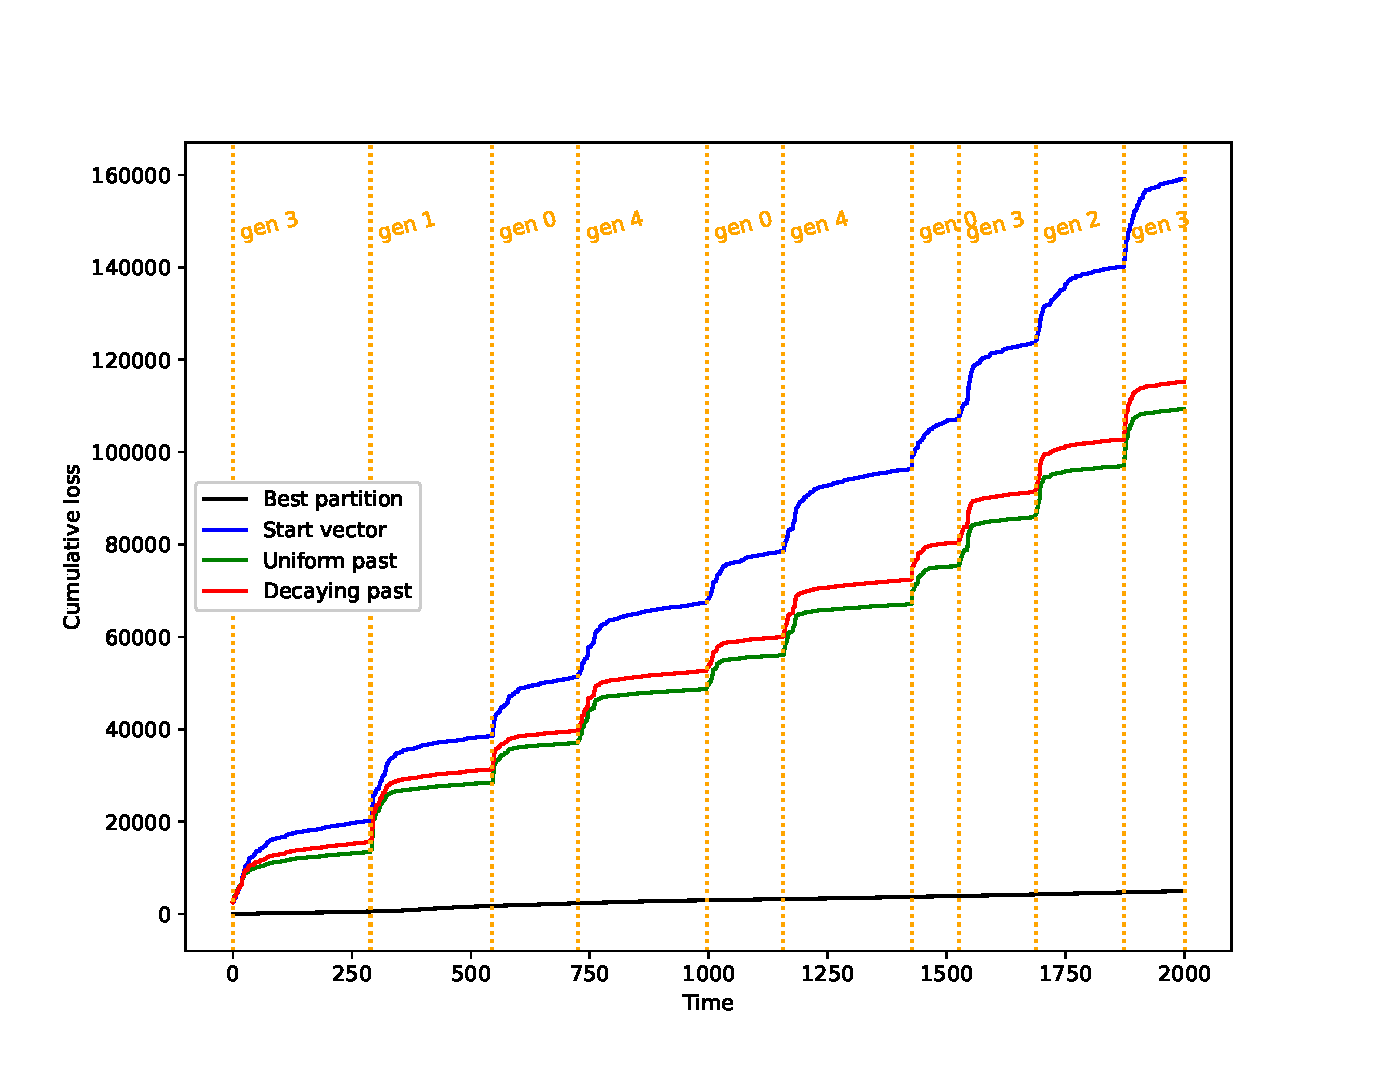
\includegraphics[width=\linewidth]{fig_52}

\begin{table}[h]
\centering
\begin{tabular}{r|cccc}
 & \multicolumn{3}{c}{Mixing scheme} \\
\toprule
{Weight function} & \centering start & \centering uniform past & \centering decaying past &  \\
\midrule
$1 / ((x + 1) * (\ln(x + 1))^2)$ & 175594.64 & 117175.93 & 122383.91 \\
$1 / (x^{1.01})$ & 132268.30 & 110569.83 & 110438.09 \\
$1 / (x^{1.1})$ & 135253.09 & 111366.88 & 111050.44 \\
$1 / (x^{1.2})$ & 137976.99 & 112298.14 & 111873.03 \\
$1 / (x^2)$ & 148080.01 & 123449.14 & 124473.63 \\
$1 / (x^{0.1})$ & 111276.08 & 117830.57 & 115101.52 \\
$1 / (x^{0.3})$ & 108946.40 & 115819.07 & 112900.36 \\
$1 / (x^{0.5})$ & 108630.68 & 114153.63 & 111221.38 \\
$1 / (x^{0.7})$ & 112027.20 & 112378.87 & 109775.49 \\
$1 / (x^{0.9})$ & 122832.21 & 110783.66 & 109408.73 \\
\bottomrule
\end{tabular}
\caption{Regret value for different Mixing Update schemes}
\end{table}



\begin{table}[h]
\centering
\begin{tabular}{r|cccc}
 &
\multicolumn{3}{c}{Weight function} \\
\toprule {$\gamma$}  &

\centering $\dfrac1{t^{1.01}}$  &
\centering $\dfrac1{t^{0.5}}$ &
\centering $\dfrac{1}{c}$  & \tabularnewline

\midrule
$0.5$ & 110151.26 & 112279.88 & 118155.78 \\
$1$ & 110438.09 & 111221.38 & 117241.85 \\
$2$ & 111563.64 & 110089.54 & 116216.44 \\
$4$ & 113922.30 & 109160.56 & 115299.68 \\
\bottomrule
\end{tabular}

\caption{Regret value for different $\gamma$ in decaying Mixing Update scheme}
\end{table}



\begin{table}[h]

\centering

\begin{tabular}{cc}
\toprule
Alpha function & regret \\
\midrule
$1 / (x + 1)$ &\ 94758.81 \\
$1 / (x + 1)^{0.5}$ & 149472.52 \\
$1 / (x + 1)^{1.5}$ &\ 92351.58 \\
$1 / (x + 1)^2)$ &\ 99120.36 \\
$1 / e^{x/3}$ &\ 99477.13 \\
$1 / (x + 10)$ &\ 94729.22 \\
$1 / (x + 100)$ &\ 94441.30 \\
$1 / (x + 1000)$ &\ 92194.36 \\
\bottomrule
\end{tabular}

\caption{Regret value for different alpha functions} \hspace{16cm}
\end{table}


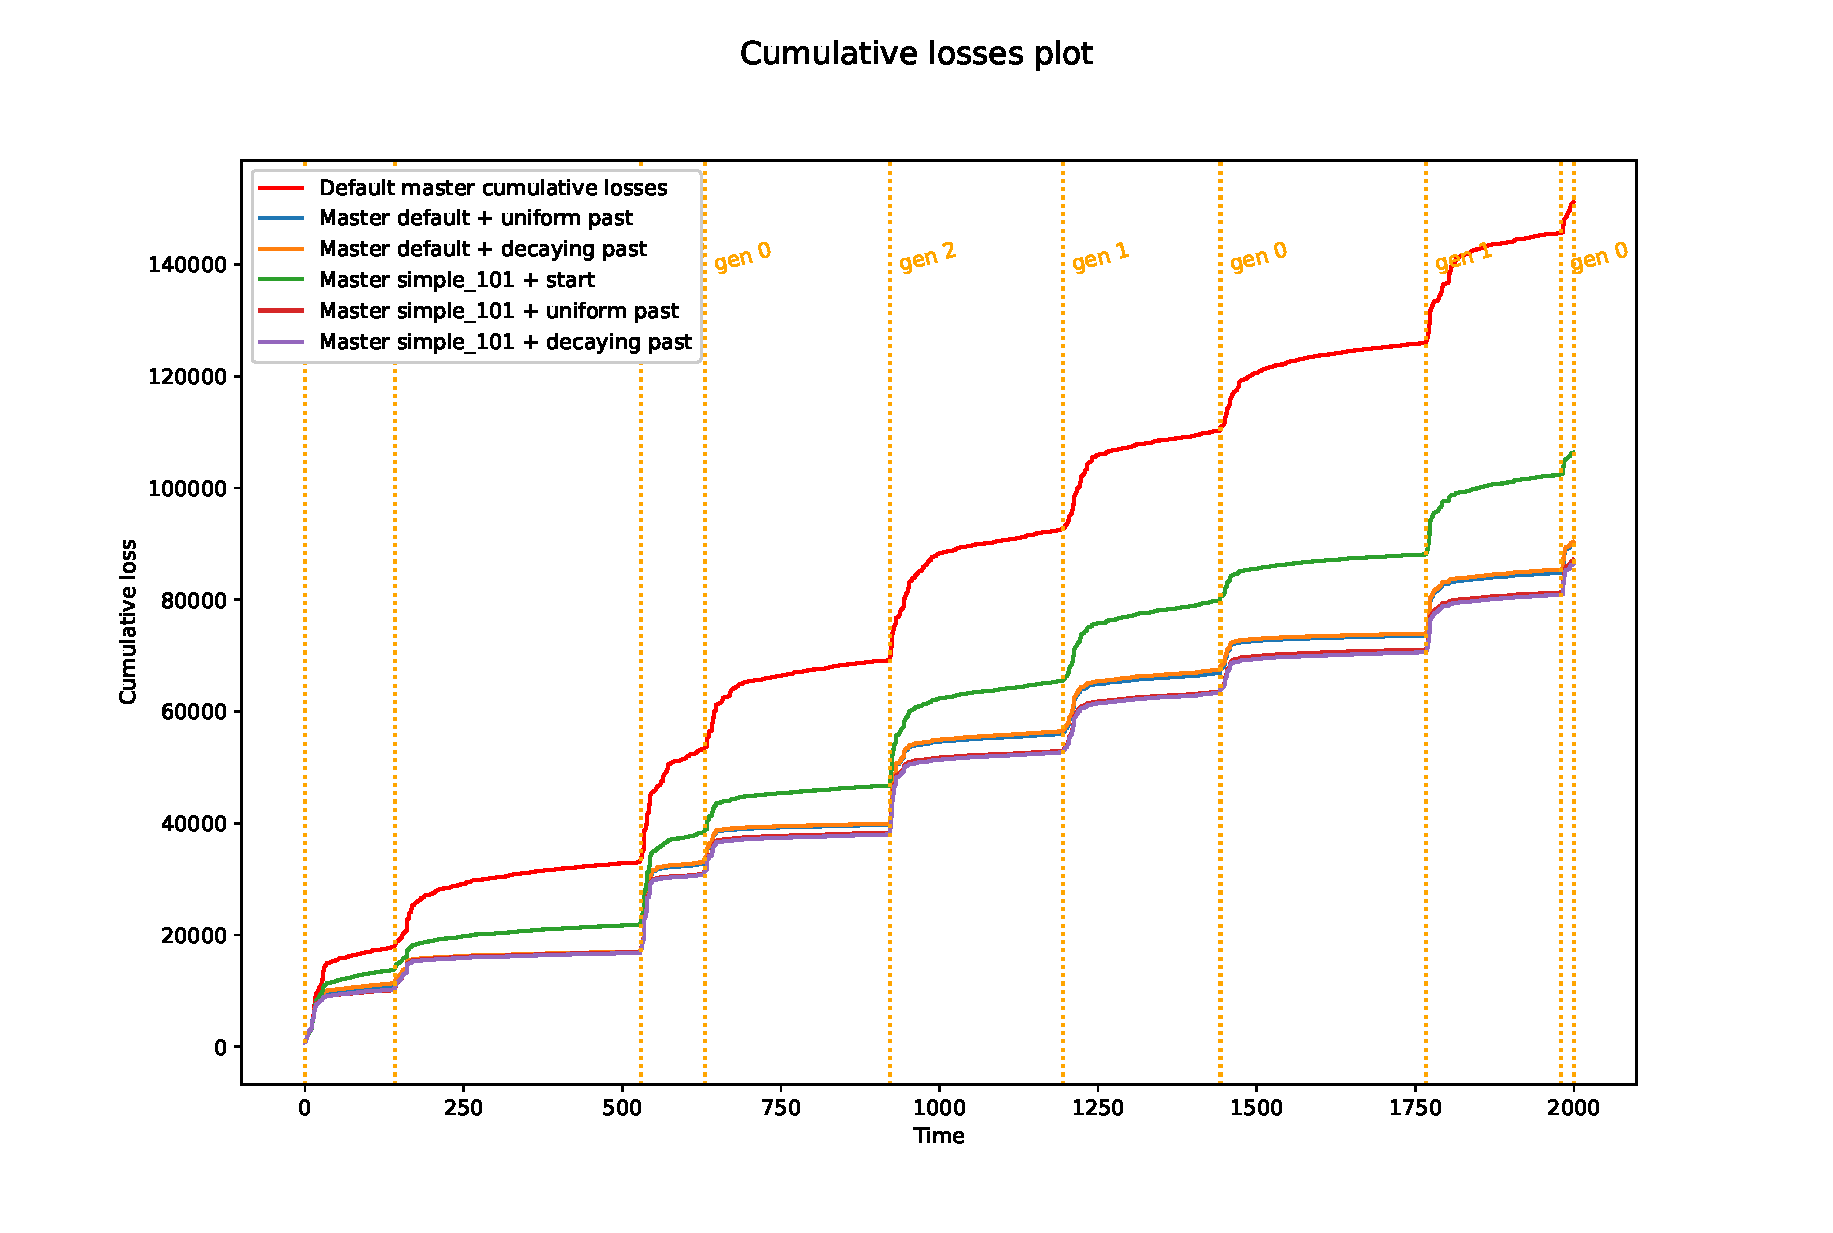
\includegraphics[width=1\linewidth]{improvement3}





\section{Conclusion}


%
%\begin{figure}[h]
%\begin{minipage}[t]{0.4\textwidth}
%
%\centering
%
%\begin{tabular}{cc}
%\toprule
%Alpha function & regret \\
%\midrule
%$1 / (x + 1)$ &\ 94758.81 \\
%$1 / (x + 1)^{0.5}$ & 149472.52 \\
%$1 / (x + 1)^{1.5}$ &\ 92351.58 \\
%$1 / (x + 1)^2)$ &\ 99120.36 \\
%$1 / e^{x/3}$ &\ 99477.13 \\
%$1 / (x + 10)$ &\ 94729.22 \\
%$1 / (x + 100)$ &\ 94441.30 \\
%$1 / (x + 1000)$ &\ 92194.36 \\
%\bottomrule
%\end{tabular}
%
%\caption{Regret value for different alpha functions} \hspace{16cm}
%
%\end{minipage}
%\hfill
%\begin{minipage}[t]{0.6\textwidth}
%% Image code goes here
%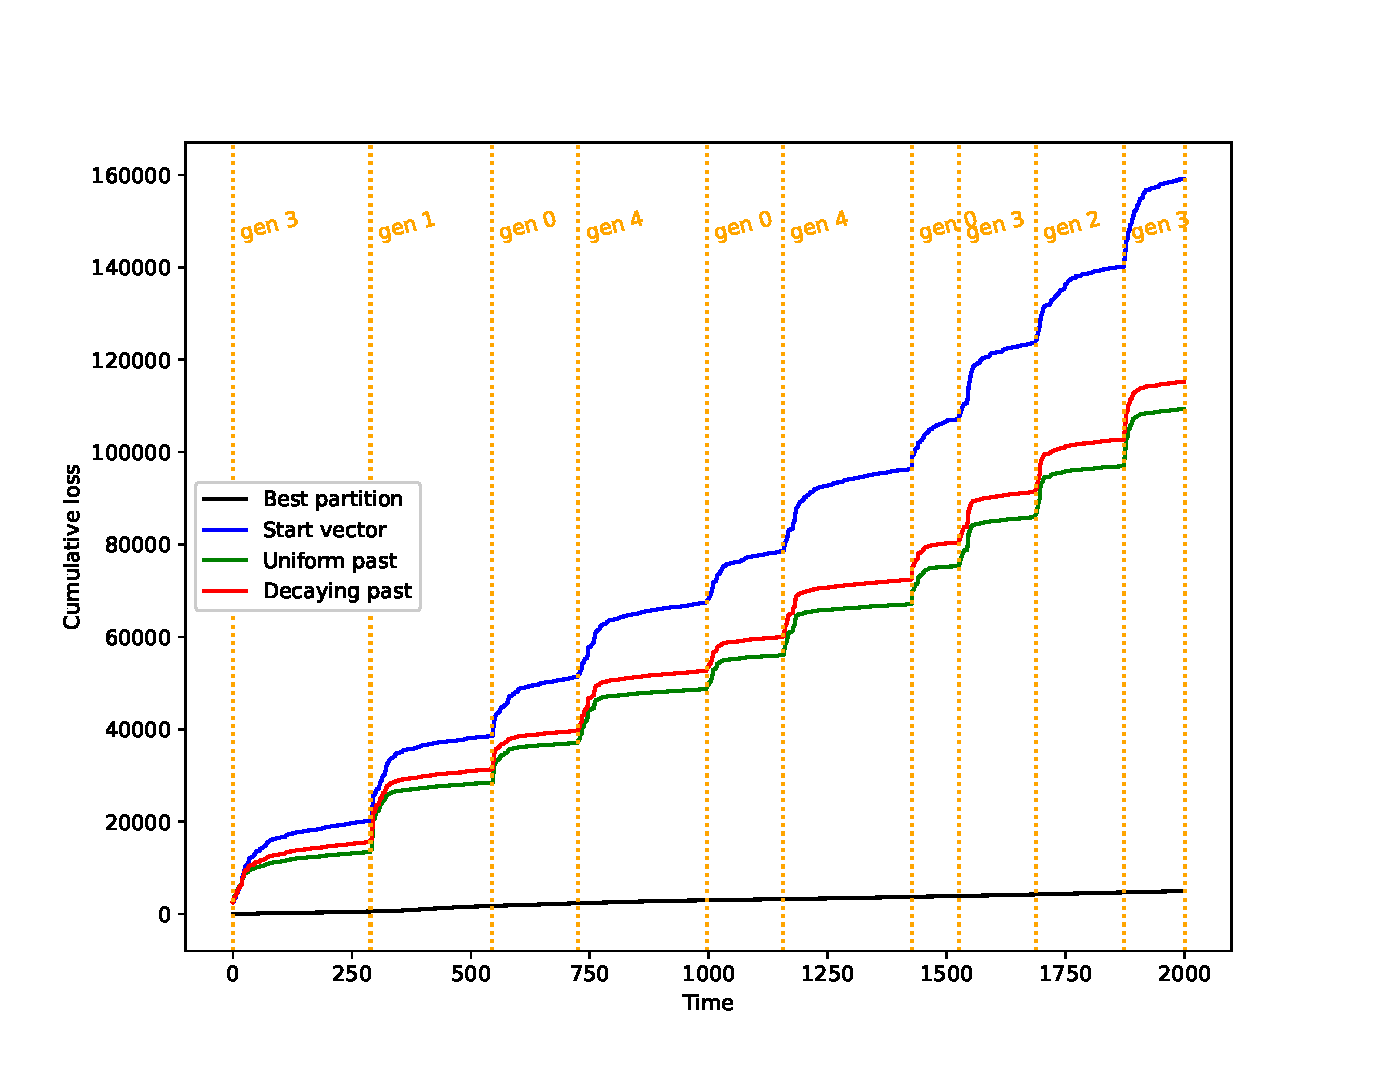
\includegraphics[width=0.7\linewidth]{fig_52}
%\caption{Comparison of algorithm performance for different mixing schemes}
%\end{minipage}
%\end{figure}


%
%\section{Preparing a manuscript}
%\noindent
%Manuscripts are prepared using \verb'jmlda.sty' style package.
%You are recommended to use \verb'jmlda_rus.bst' and \verb'jmlda_eng.bst' style files for generating bibliography using Bib\TeX.
%
%Visit the \url{http://jmlda.org/?lang=en} website for detailed submission instructions, templates and other information.
%
%Please note that this file must be saved in~\verb'UTF-8' encoding. Where possible select~\verb'UTF-8 without BOM' encoding. 
%To change the encoding please use \verb'Sublime Text' or \verb'Notepad++' text editors.
%
%\section{Structure of the article}
%\noindent
%Divide your article into clearly defined and numbered sections and paragraphs.

%\section{Concluding Remarks}
%This section should provide the summary and explore the significance of the results achieved and list problems not yet solved.
%Results should be clear and concise.

%%%% please specify doi of the cited item if possible, see~\bibitem{article}
%%%% Crossref doi of the item can be retrieved at http://www.crossref.org/guestquery/

\begin{thebibliography}{99}

\bibitem{book}
    \BibAuthor{N.\,Cesa-Bianchi, G.\,Lugosi}. 2006.
    \BibTitle{Prediction, Learning, and Games}.
    Available at: \BibUrl{https://ii.uni.wroc.pl/~lukstafi/pmwiki/uploads/AGT/Prediction_Learning_and_Games.pdf}
    
\bibitem{ebook}
    \BibAuthor{Hyndman,\,R.\,J. \& Athanasopoulos,\,G., 2nd edition}. 2018.
    \BibTitle{Forecasting: Principles and Practice}.
    \BibJournal{OTexts: Melbourne, Australia} .
    Available at: \BibUrl{https://otexts.com/fpp2/}
    
    
\bibitem{vvbook}
    \BibAuthor{V.\,V'yugin}. 2022.
    Matematicheskie osnovy mashinnogo obucheniya i prognozirovaniya 
    [Mathematical Foundations of Machine Learning and Forecasting].
    Available at: \BibUrl{http://iitp.ru/upload/publications/6256/vyugin1.pdf}

\bibitem{article}
    \BibAuthor{V.\,V’yugin, V.\,Trunov}. 2023.
    Prognozirovanie lokal'no statsionarnykh dannykh s ispol'zovaniem predskazanii ekspertnykh strategiy
    [Prediction of Locally Stationary Data Using Prediction with
Expert Advice].
    Available at: \BibUrl{http://www.jip.ru/2023/470-487-2023.pdf}
    
\bibitem{article98}
    \BibAuthor{M.\,Herbster, M.\,Warmuth}. 1998.
    \BibTitle{Tracking the best expert}.
    Available at: \BibUrl{https://link.springer.com/content/pdf/10.1023/A:1007424614876.pdf}
    
\bibitem{article02}
    \BibAuthor{O.\,Bousquet, M.\,Warmuth}. 2002.
    \BibTitle{Tracking a small set of experts by mixing past posteriors}.
    Available at: \BibUrl{https://www.jmlr.org/papers/volume3/bousquet02b/bousquet02b.pdf}
%
%
%\bibitem{webArticle}
%   \BibAuthor{Blaga,~P.\,A.} 2007.
%   Commutative Diagrams with XY-pic II. Frames and Matrices.
%   \BibJournal{PracTEX J.}  4.
%   Available at: \BibUrl{https://tug.org/pracjourn/2007-1/blaga/blaga.pdf}
%    (accessed February 20, 2007).
%
%\bibitem{webResource}
%   XYpic.
%   Available at: \BibUrl{http://akagi.ms.u-tokyo.ac.jp/input9.pdf}
%   (accessed April 09, 2015).
%
%\bibitem{inproceedingsRus}
%   \BibAuthor{Usmanov,~T.\,S., A.\,A.~Gusmanov, I.\,Z.~Mullagalin, R.\,Yu.~Mukhametshina, A.\,N.~Chervyakova, and A.\,V.~Sveshnikov.} 2007.
%   Osobennosti proektirovaniya razrabotki mestorozhdeniy s primeneniem gidrorazryva plasta
%   [Features of the design of field development with the use of hydraulic fracturing].
%   \BibJournal{6th Symposium (International) ``New Energy Saving Subsoil Technologies and the
%   Increasing of the Oil and Gas Impact'' Proceedings}.
%   Moscow:~Publisher. 267--272. (In Russian)
%       
%\bibitem{inproceedingsEng}
%    \BibAuthor{Author,~N.} 2009.
%    Paper title.
%    \BibJournal{10th Conference (International) on Any Science Proceedings}.
%    Place of publication: Publisher. 111--122.
%   
%\bibitem{techreport}
%   \BibAuthor{Lambert,~P.} 1993.
%   \BibTitle{The title of the work}.
%   Place of publication:~The institution that published.  Report~2.
            
\end{thebibliography}

\end{document}
